\documentclass[12pt]{article}

\title{Pattern Recognition Homework 2}
\author{Kosate Limpongsa \\ kosatelim@gmail.com}

\usepackage{amsmath,amsthm,mathtools}
\usepackage{graphicx}
\usepackage{float}
\usepackage{listings}
\usepackage{hyperref}
\graphicspath{ {images/} }
\begin{document}

\maketitle

\section{MLE}

\begin{align*}
  y_2 = \alpha y_1 + w_1 &\qquad w_0, w_1 \sim N(0, \sigma^2) \\
  y_1 = \alpha y_0 + w_0 &\qquad y_0 \sim N(0, \lambda)
\end{align*}
\begin{center}
Find $\operatorname*{argmax}_\alpha p(y_2,y_1,y_0|\alpha)$
\end{center}
\begin{align*}
p(y_2,y_1,y_0|\alpha) ={} & p(y_2|y_1,y_0,\alpha) \, p(y_1|y_0, \alpha) \, p(y_0|\alpha) \\
p(y_n|y_{n-1}, y_{n-2}, ...) ={} & p(y_n|y_{n-1}) \\
p(y_2,y_1,y_0|\alpha) ={} & p(y_2|y_1, \alpha) \, p(y_1|y_0, \alpha) \, p(y_0|\alpha)
\end{align*}
\begin{align*}
\begin{split}
p(y_2,y_1,y_0|\alpha) ={} 
  & \frac{1}{\sqrt{2\pi\sigma^2}}exp(-\frac{(y_2-\alpha y_1)^2}{2 \sigma^2}) \\
  & \frac{1}{\sqrt{2\pi\sigma^2}}exp(-\frac{(y_1-\alpha y_0)^2}{2 \sigma^2}) \\
  & \frac{1}{\sqrt{2\pi\lambda}}exp(-\frac{y_0^2}{2 \lambda})
\end{split}
\\
log p(y_2,y_1,y_0|\alpha) ={} 
  & -\frac{1}{2}log\sqrt{2\pi\sigma^2} - \frac{(y_2-\alpha y_1)^2}{2 \sigma^2} \\
  & -\frac{1}{2}log\sqrt{2\pi\sigma^2} - \frac{(y_1-\alpha y_0)^2}{2 \sigma^2} \\
  & -\frac{1}{2}log\sqrt{2\pi\lambda} - \frac{y_0^2}{2 \lambda}
\\
\frac{\partial log p(y_2,y_1,y_0|\alpha)}{\partial \alpha} ={}
  & \frac{y_2 y_1}{\sigma^2} - \frac{\alpha y_1^2}{\sigma^2} +
  \frac{y_1 y_0}{\sigma^2} - \frac{\alpha y_0^2}{\sigma^2}
\end{align*}
Find MLE by taking $\frac{\partial log P}{\partial \alpha} = 0$
\begin{align*}
  \frac{\partial log p(y_2,y_1,y_0|\alpha)}{\partial \alpha} ={} & 0\\
  0 ={} & \frac{y_2 y_1 - \alpha y_1^2 + y_1 y_0 - \alpha y_0^2}{\sigma^2} \\
  0 ={} & y_2 y_1 - \alpha y_1^2 + y_1 y_0 - \alpha y_0^2 \\
  \alpha ={} & \frac{y_2 y_1 - y_1 y_0}{y_1^2 + y_2^2}
\end{align*}

\section{Simple Bayes Classifier}
\label{sec:bayes}

\subsection{Plot posteriors of $N(5,2)$ and $N(0,2)$}
\begin{figure}[ht]
  \centering
  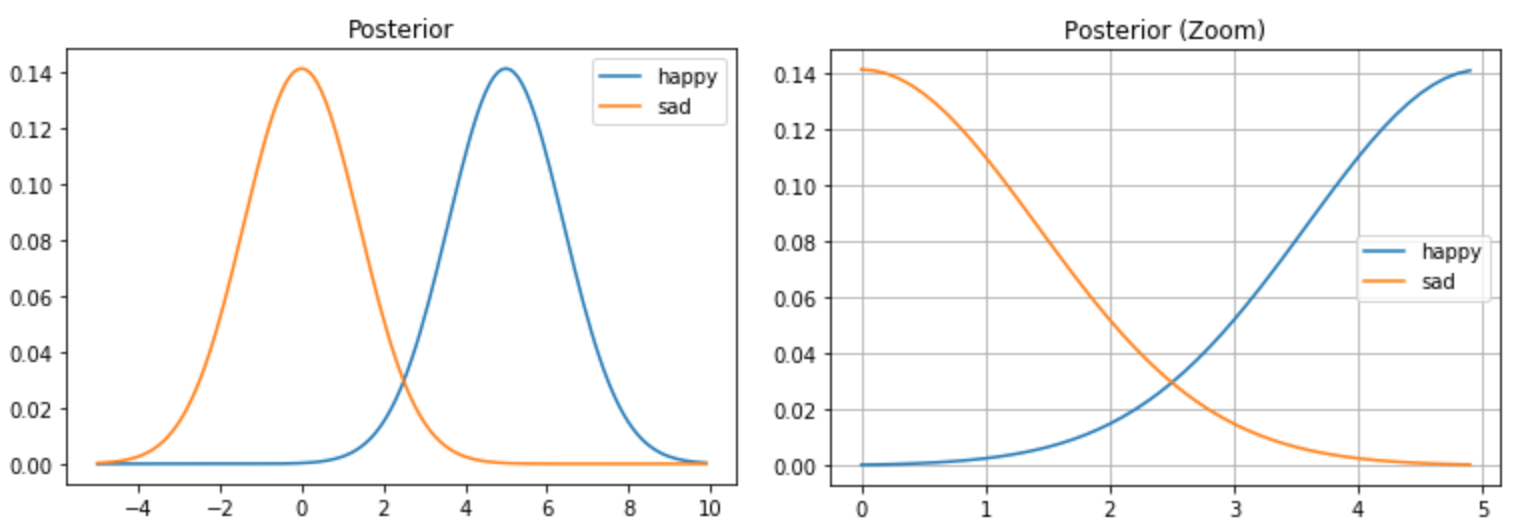
\includegraphics[width=1\textwidth]{bayes-1.png}
  \end{figure}
As you see, the decision boundary of $N(5,2)$ and $N(0,2)$ $= 2.5$

\begin{align*}
P(x|w_1) \, P(w_1) &= P(x|w_2) \, P(w_2) \\
P(x | w_1) &= P(w | x_2) \\
(\frac{1}{\sqrt{2 \pi \sigma_1^2}}) \, exp (-\frac{(x-\mu_1)^2}{2 \sigma_1^2}) &= (\frac{1}{\sqrt{2 \pi \sigma_2^2}}) \, exp (-\frac{(x-\mu_2)^2}{2 \sigma_2^2}) \\
  \text{Since } \sigma_1 &= \sigma_2 \\
  (x-\mu_1)^2 &= (x-\mu_2)^2 \\
  x^2 - 2 x \mu_1 + \mu_1^2 &= x^2 - 2 x \mu_2 + \mu_2^2 \\
  -10x + 25 &= 0 \\
  x &= 2.5
\end{align*}

\subsection{What happens if prior of happy cat is $0.8$}

\begin{figure}[ht]
  \centering
  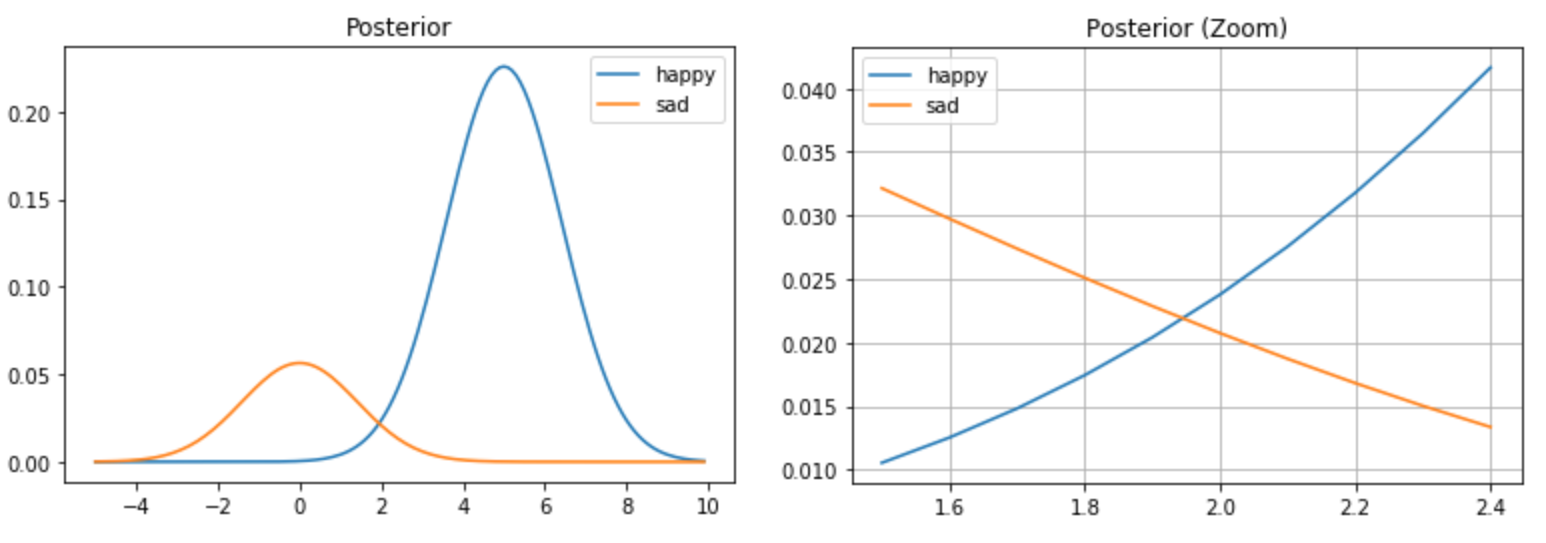
\includegraphics[width=1\textwidth]{bayes-2.png}
  \end{figure}
As you see, the decision boundary of $N(5,2)$ and $N(0,2)$ $\approx 1.95$

\begin{align*}
  P(x|w_1) \, P(w_1) &= P(x|w_2) \, P(w_2) \\
  (\frac{1}{\sqrt{2 \pi \sigma_1^2}}) \, exp (-\frac{(x-\mu_1)^2}{2 \sigma_1^2}) (0.8) &= (\frac{1}{\sqrt{2 \pi \sigma_2^2}}) \, exp (-\frac{(x-\mu_2)^2}{2 \sigma_2^2}) (0.5) \\
  exp (-\frac{(x-5)^2}{4}) 4 &= exp (-\frac{x^2}{4}) \\
  -\frac{(x - 5)^2}{8} + ln 4 &= -\frac{x^2}{8} \\
  x &= \frac{25 - 4 log 4}{10} \\
  x &\approx 1.9454
  \end{align*}

\subsection{Plot $P(x|w_1) = N(5,2), P(x|w_2) = N(0,4)$}

\begin{figure}[ht]
  \centering
  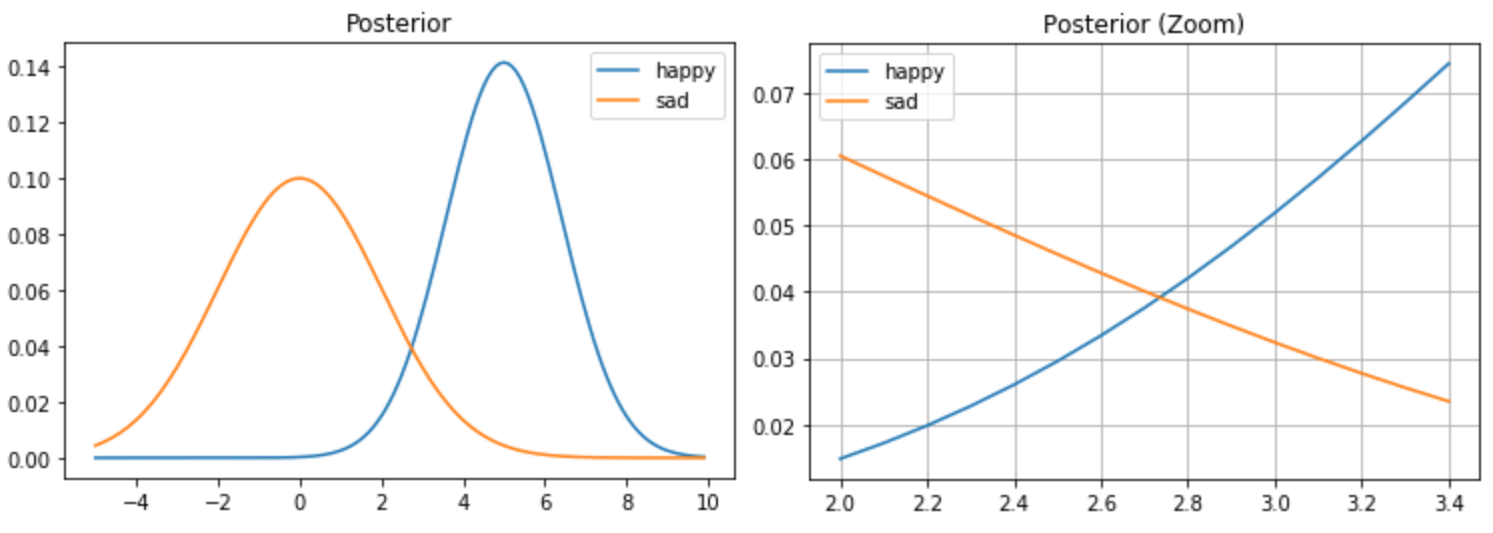
\includegraphics[width=1\textwidth]{bayes-3.png}
  \end{figure}

As you see, the decision boundary when change prior of happy cat $\approx 2.74$

\begin{align*}
  P(x|w_1) \, P(w_1) &= P(x|w_2) \, P(w_2) \\
  \text{Since } P(w_1) &= P(w_2) \\
  P(x|w_1) &= P(x|w_2) \\
  (\frac{1}{\sqrt{2 \pi \sigma_1^2}}) \, exp (-\frac{(x-\mu_1)^2}{2 \sigma_1^2}) &= (\frac{1}{\sqrt{2 \pi \sigma_2^2}}) \, exp (-\frac{(x-\mu_2)^2}{2 \sigma_2^2}) \\
  (\frac{1}{\sqrt{4 \pi}}) \, exp (-\frac{(x-5)^2}{4}) &= (\frac{1}{\sqrt{8 \pi}}) \, exp (-\frac{x^2}{8}) \\
  log\sqrt{2} - \frac{x^2 - 10x + 25}{4} &= -\frac{x^2}{8} \\
  8log\sqrt{2} - 50 &= x(x - 20) \\
  x &= 10 - \sqrt{50 + log16} \\
  x &\approx 2.7355
\end{align*}

% \subsection{(Optional) Prove decision boundary is $x = \frac{\mu_1 + \mu_2}{2}$}

\begin{align*}
  P(x|w_1) \, P(w_1) &= P(x|w_2) \, P(w_2) \\
  \text{Since } P(w_1) &= P(w_2) = 0.5 \\
  P(x|w_1) &= P(x|w_2) \\
  (\frac{1}{\sqrt{2 \pi \sigma^2}}) \, exp (-\frac{(x-\mu_1)^2}{2 \sigma^2}) &= (\frac{1}{\sqrt{2 \pi \sigma^2}}) \, exp (-\frac{(x-\mu_2)^2}{2 \sigma^2}) \\
  x^2 - 2x\mu_1 + \mu_1^2 &= x^2 - 2x\mu_2 + \mu_2^2 \\
  x &= \frac{\mu_2^2 - \mu_1^2}{2\mu_2 - 2\mu_1} \\
  x &= \frac{(\mu_2^2 - \mu_1^2)(\mu_2 + \mu_1)}{2(\mu_2 - \mu_1)(\mu_2 + \mu_1)} \\
  x &= \frac{\mu_2 + \mu_1}{2}
\end{align*}


\section{Housekeeping Genes Prediction}

\subsection{Data Items}
How many items are NaN in the $is\_hk$ column? How many items are known
housekeeping genes? How many items are known tissue specific genes?
  \begin{figure}[H]
    \noindent\makebox[\textwidth]{
      \setlength{\fboxsep}{0pt}\fbox{
        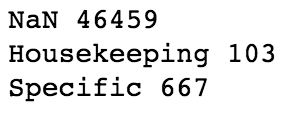
\includegraphics[width=0.2\paperwidth]{hk_count.png}
      }
    }
    \end{figure}
\subsection{Observe Histogram}
Observe the histograms. Can we use a Gaussian to estimate this histogram?
Why? What about a Gaussian Mixture Model (GMM)?

\begin{figure}[H]
  \centering
  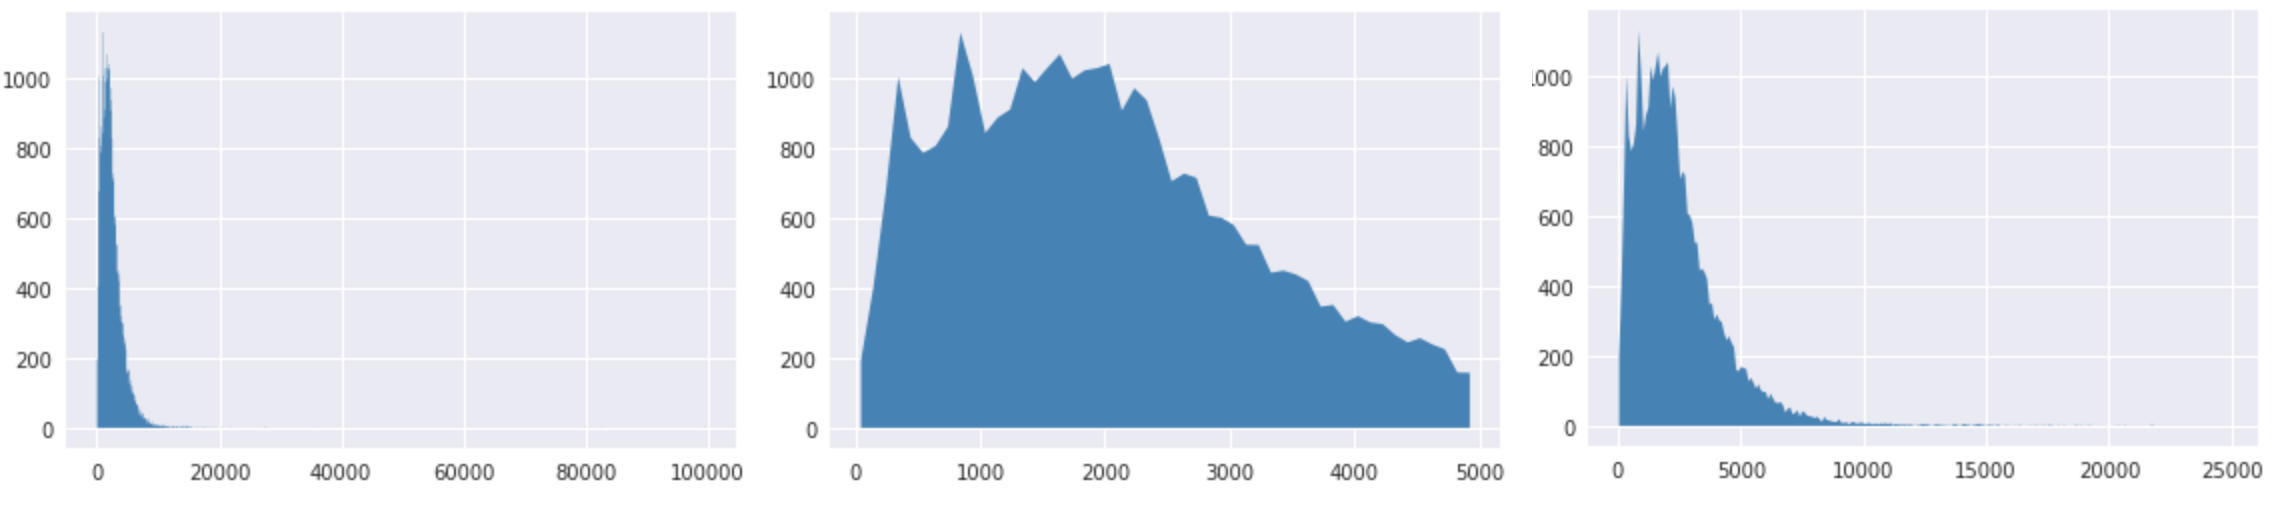
\includegraphics[width=1\textwidth]{cdn_before.png}
  \end{figure}

We should not use Gaussian to estimate this histogram because there are some little details that
Gaussian could not capture. I think it can archive very high accuracy with only single Gaussian but if you want to boost up some accuracy. 
So it is better to use GMM that can capture some complex curve inside these information.

\subsection{Zero Bins}
How many bins have zero counts? Do you think this is a good discretization?
Why?

\begin{figure}[H]
  \noindent\makebox[\textwidth]{
    \setlength{\fboxsep}{0pt}\fbox{
      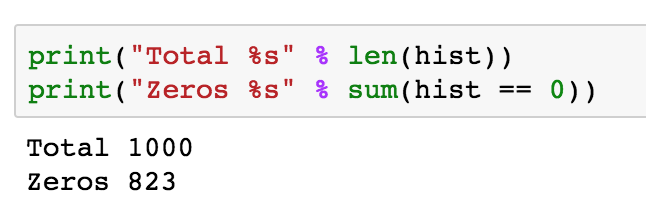
\includegraphics[width=0.4\paperwidth]{hk_zero_bins.png}
    }
  }
  \end{figure}

The number of zero bins is about 82.3\% of total amount of bins. It is not a good discretization
because amount of bin that include zero are too much.

\subsection{New Discretization}

Plot the histogram according to our new discretization scheme just like the
process above (with ∼1000 bins, and show 3 plots). Does it come out like how
it should be?

\begin{figure}[H]
  \noindent\par
  \raisebox{-.5\height}{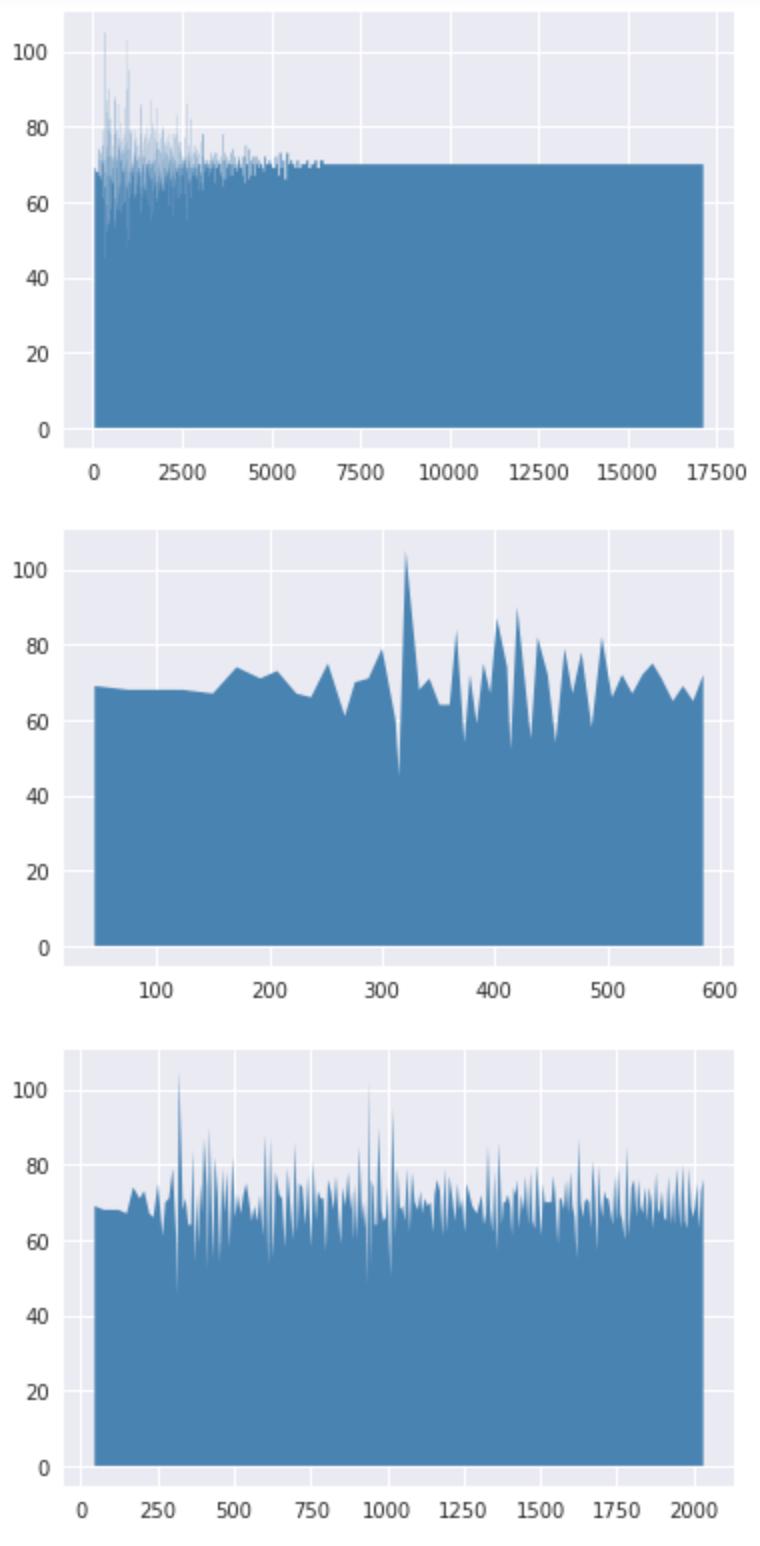
\includegraphics[width=0.48\textwidth]{cdna.png}}%
  \hfill
  \raisebox{-.5\height}{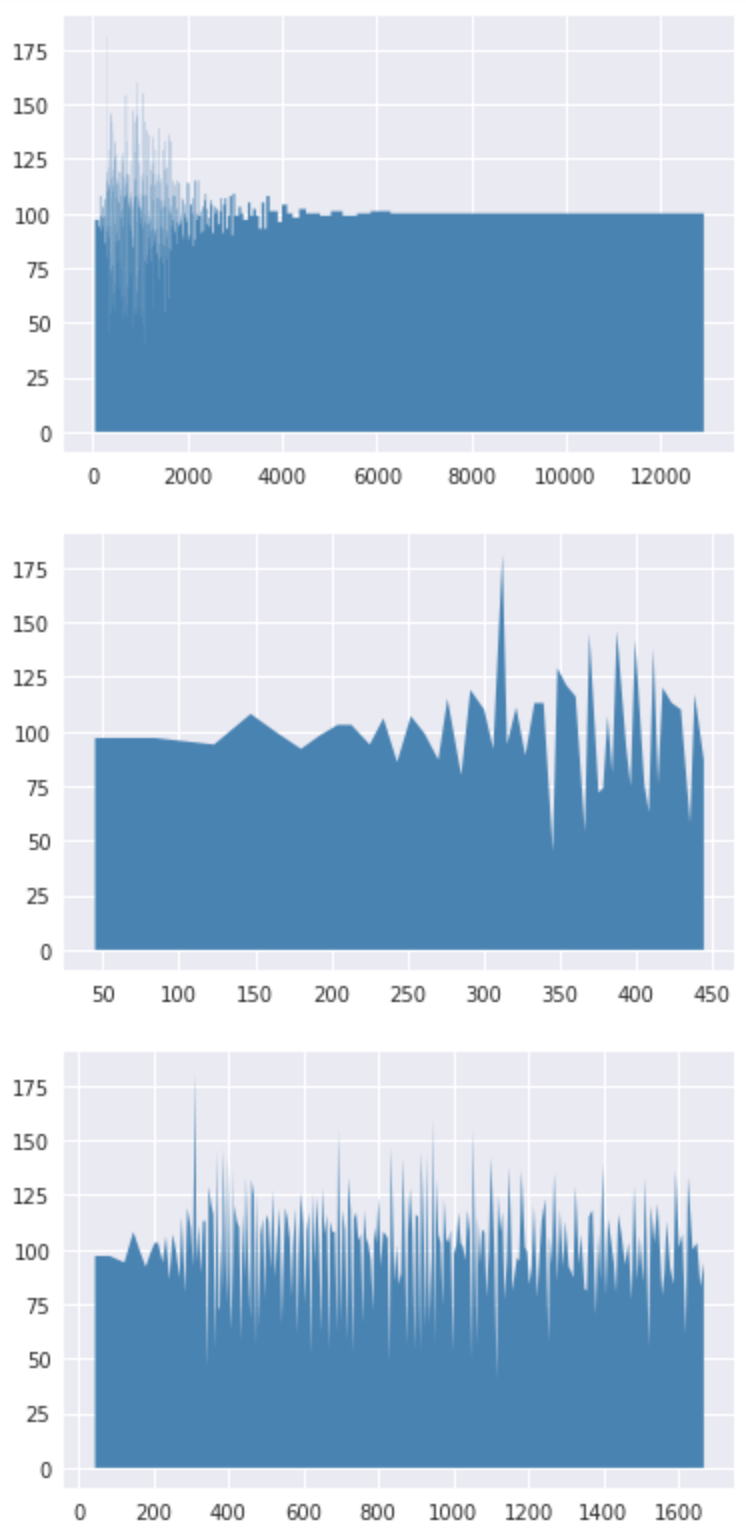
\includegraphics[width=0.47\textwidth]{cds.png}}%
  \par
  \caption{(Left) cDNA density plot with 70 spacing (Right) CDS density plot with 100 spacing}
  \end{figure}

It does come out like how it should be. The first half of data is swing while the other half are normal uniform,
which is similar to the first plot that first half of data contain a lot of data (It is easiler to swing) and other half has no data.

\subsection{Likehood Distribution}

What is the MLE for the likelihood distributions of each of the 9 features? Plot
the likelihood distributions.

\begin{figure}[H]
  \centering
  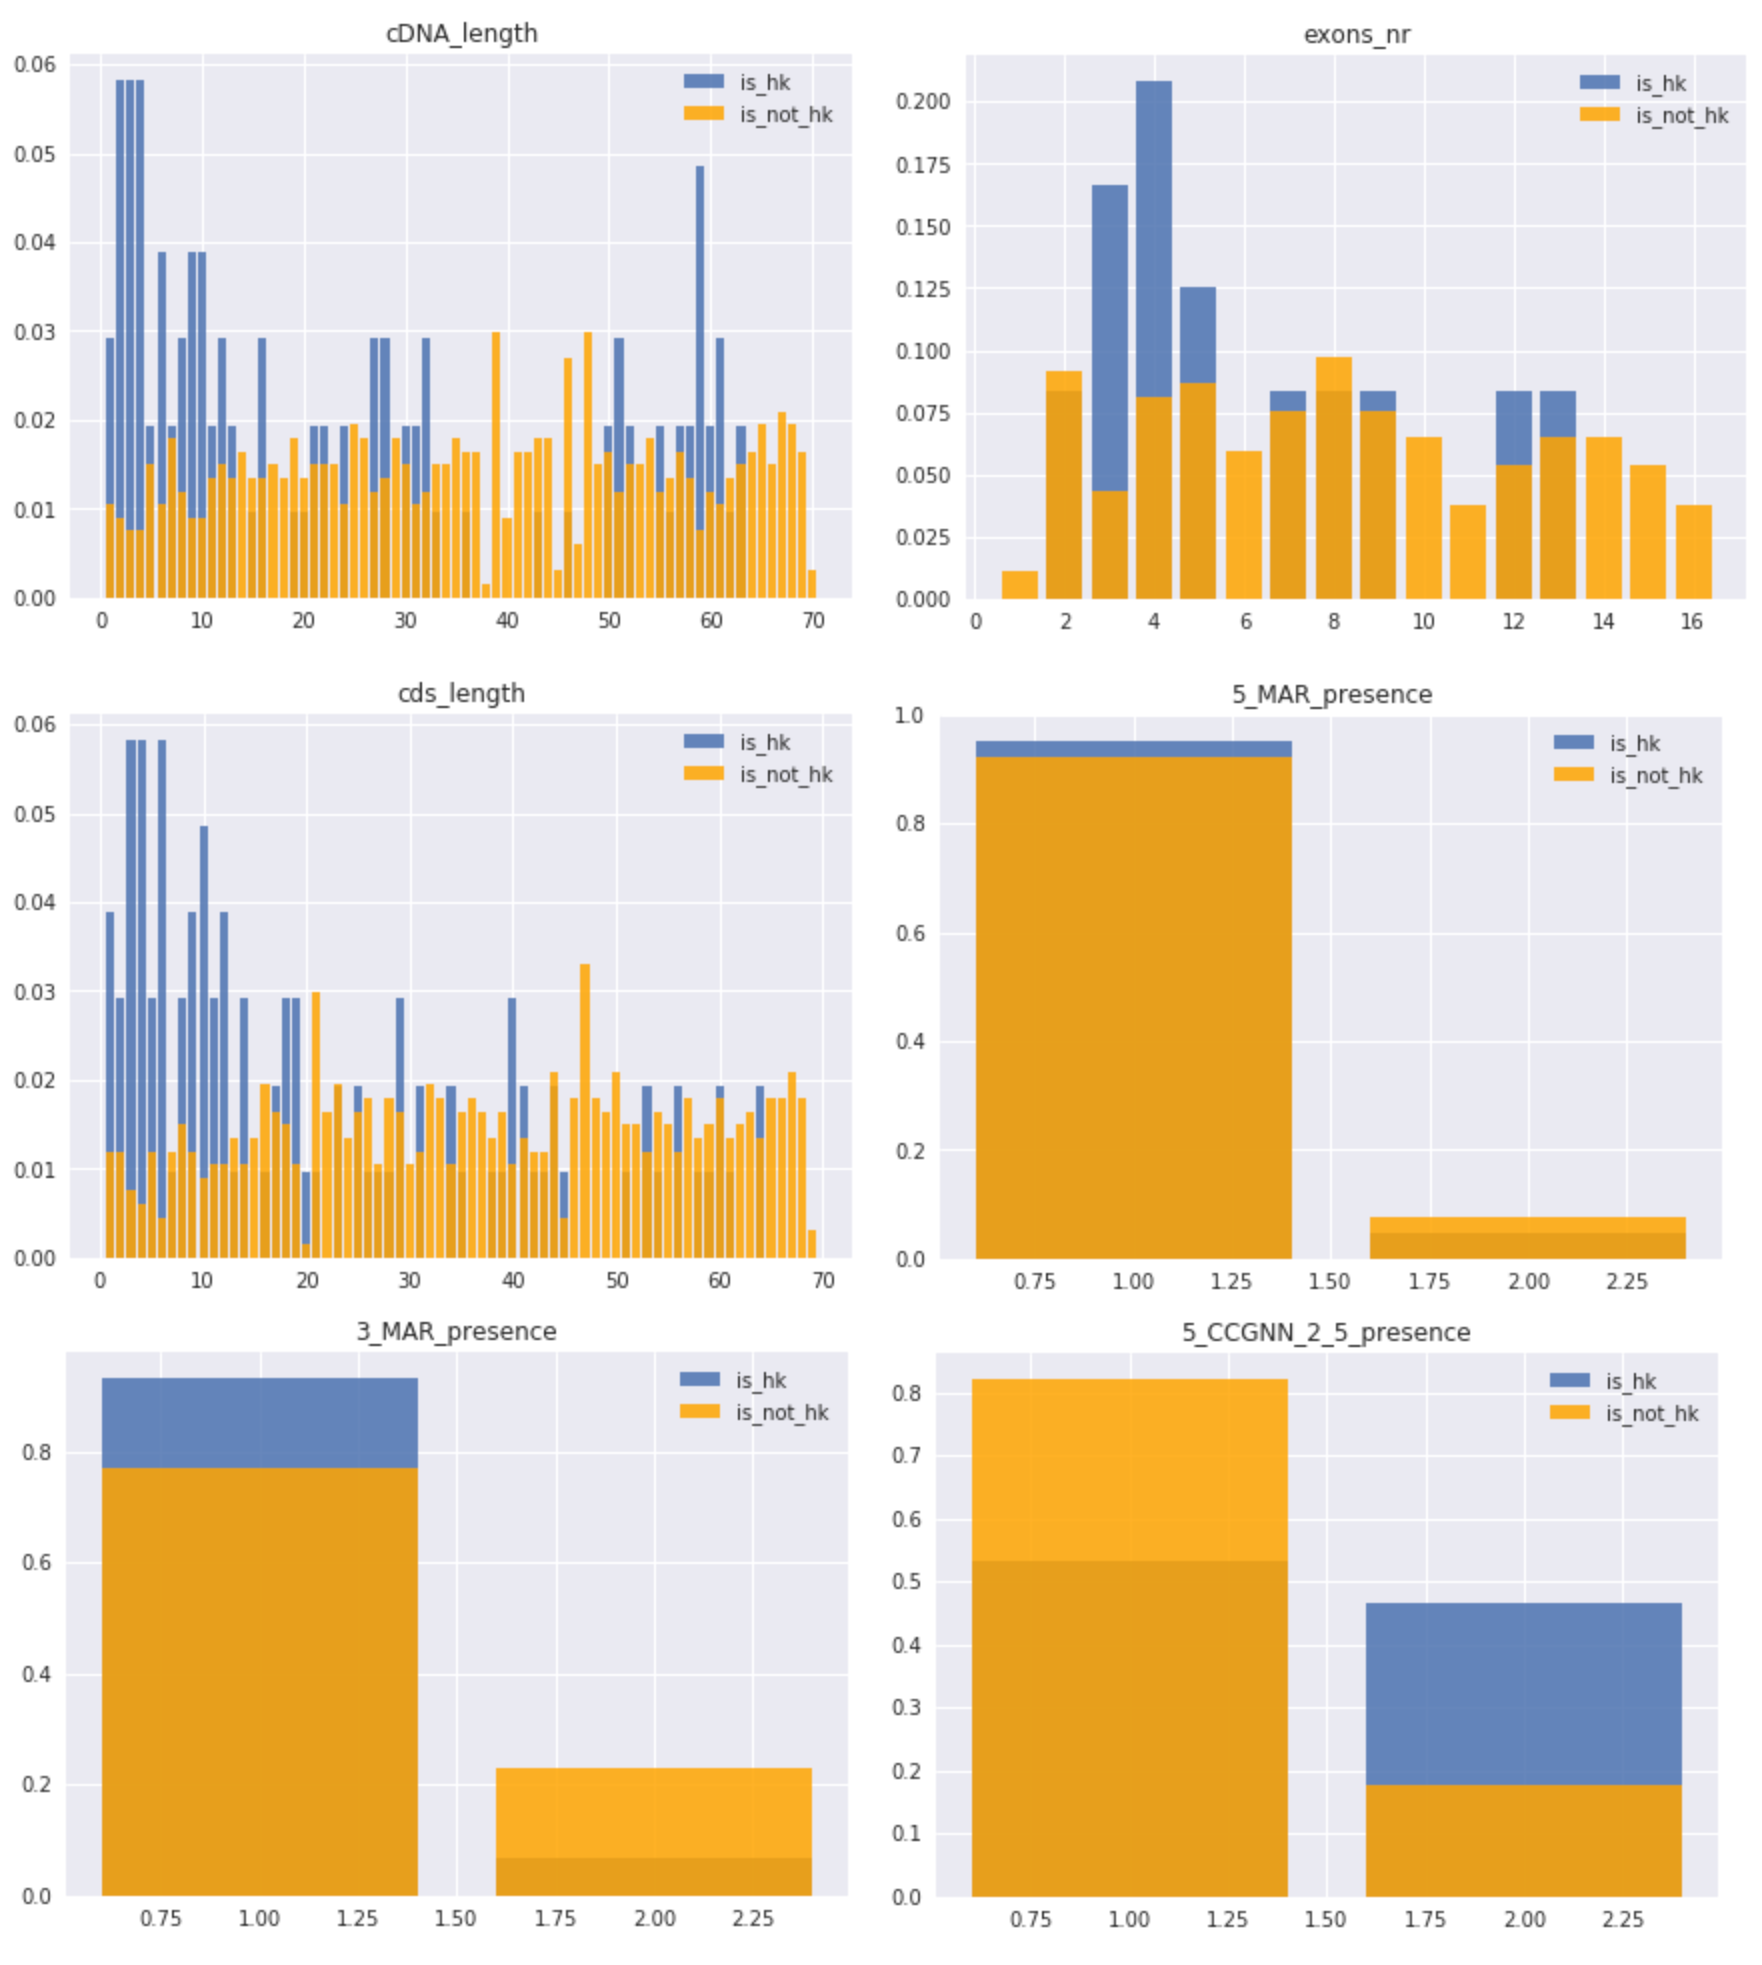
\includegraphics[width=1\textwidth]{mle_1.png}
  \end{figure}

\begin{figure}[H]
  \centering
  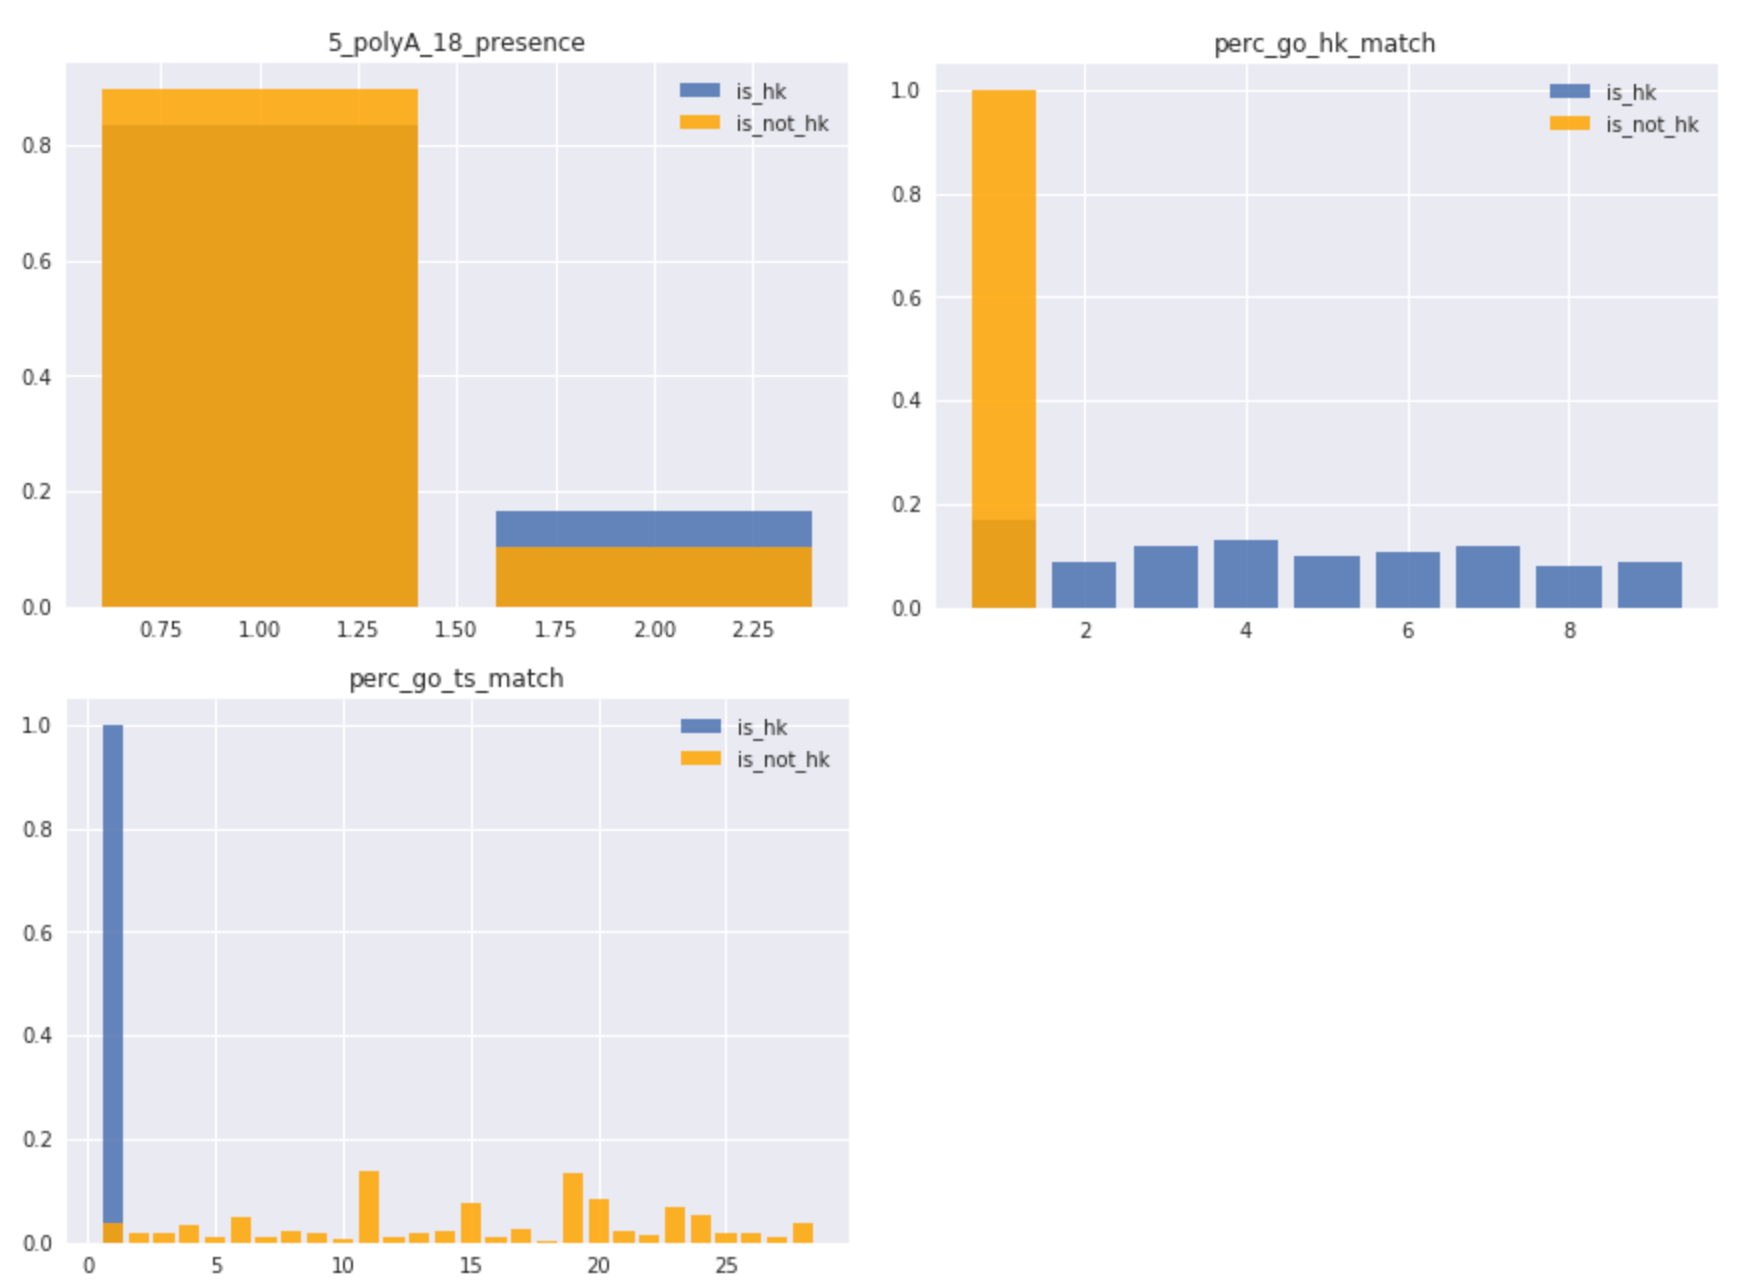
\includegraphics[width=1\textwidth]{mle_2.png}
  \end{figure}

\subsection{Prior}
What is the prior distribution of the two classes?
\begin{align*}
P(is\_hk) &= 0.133766 \\
P(is\_not\_hk) &= 0.866234
\end{align*}

\subsection{Prediction}
Use the learned distributions to classify the test set. Don’t forget to allow
your classifier to handle missing values in the test set. Report the overall
Accuracy. Then, report the Precision, Recall, and F score for detecting
housekeeping gene.
\begin{align*}
Accuracy &= 0.987179 \\
Precision &= 0.916667 \\
Recall &= 1.000000 \\
F1 &= 0.956522 \\
\end{align*}

\subsection{Baseline Random Choice}
The random choice baseline is the accuracy if you make a random guess for
each test sample. Give random guess (50\% being housekeeping, and 50\%
being not housekeeping) to the test samples. Report the overall Accuracy.
Then, report the Precision, Recall, and F score for detecting housekeeping
gene using the random choice baseline
\begin{align*}
Accuracy &= 0.525641 \\
Precision &= 0.175000 \\
Recall &= 0.636364 \\
F1 &= 0.274510
\end{align*}

\subsection{Baseline Majority}
The majority rule is the accuracy if you use the most frequent class from the
training set as the classification decision. Report the overall Accuracy. Then,
report the Precision, Recall, and F score for detecting housekeeping gene using
the majority rule baseline.
\begin{align*}
Accuracy &= 0.858974 \\
Precision &= 0.000000 \\
Recall &= 0.000000 \\
F1 &= 0.000000
\end{align*}

\begin{tabular}{l*{4}{c}r}
  Algorithm              & Accuracy & Precision & Recall & F1 \\
  \hline
  Random Choice   & 52.56 & 17.50 & 63.64  & 27.45  \\
  Majority        & 85.90 & 0.00  & 0.00   & 0.00  \\
  Naive Bayes     & 98.72 & 91.67 & 100.00 & 95.65  \\
  \end{tabular}

\subsection{Threshold Value}
Use the following threshold values
$t = np.arange(-5,5,0.05)$
find the best accuracy, and F score (and the corresponding thresholds)

\begin{figure}[H]
  \noindent\makebox[\textwidth]{
    \setlength{\fboxsep}{0pt}\fbox{
      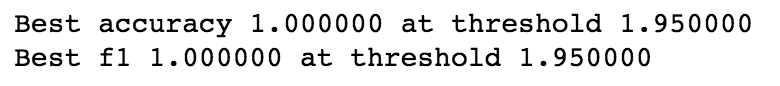
\includegraphics[width=0.45\paperwidth]{best_acc.png}
    }
  }
  \end{figure}

\subsection{RoC}
Plot the RoC of your classifier.

\begin{figure}[H]
  \centering
  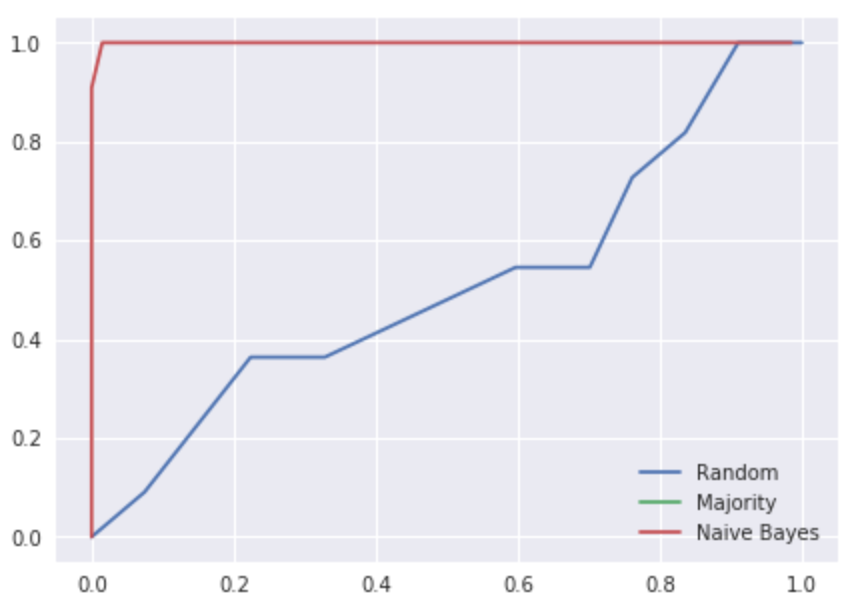
\includegraphics[width=0.8\textwidth]{roc_less.png}
  \end{figure}

\subsection{RoC with different bin size}
Change the number of discretization bins from ${\sim}1000$ to ${\sim}500$. What happens to the RoC curve? Which discretization is better? The number of discretization bins can be considered as a hyperparameter, and must be chosen by comparing the final performance.

\begin{figure}[H]
  \noindent\par
  \raisebox{-.5\height}{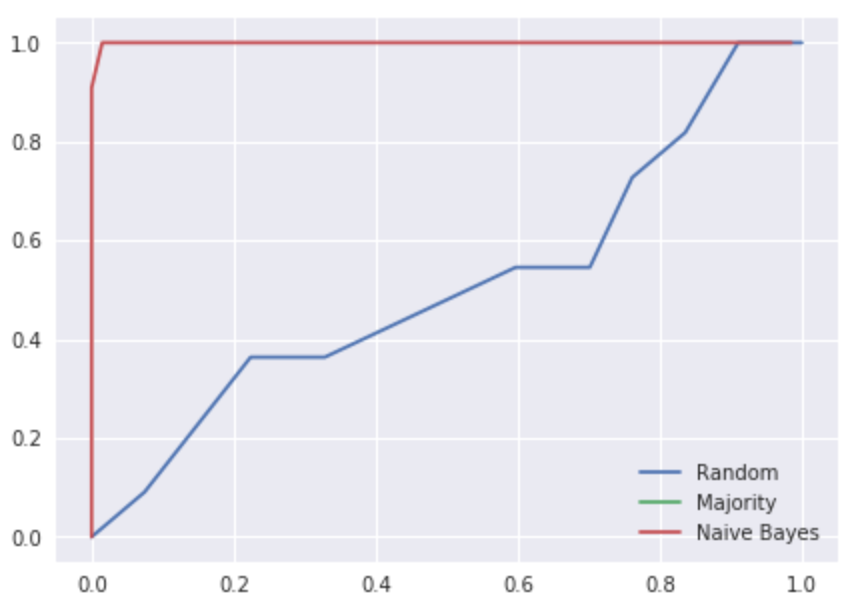
\includegraphics[width=0.48\textwidth]{roc_less.png}}%
  \hfill
  \raisebox{-.5\height}{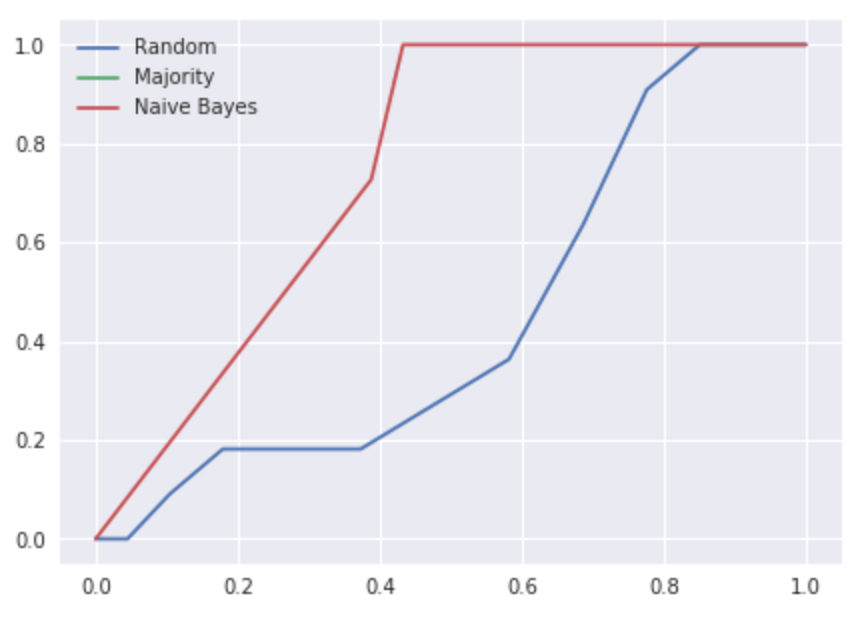
\includegraphics[width=0.49\textwidth]{roc_much.png}}%
  \par
  \caption{(Left) ROC of ${\sim}1000$ bins (Right) ROC of ${\sim}50$ bins}
  \end{figure}

The RoC curve with large amount of bins is trend to be more beautiful than the curve with less bins data.
We will see if we decrease the size of decreatization bins, the true positive rate will be decrease,
and errors will be increase, which cause the accuracy of train dataset to be drop-off.

\section*{Code Submission}

I have submitted 4 files of code consist of:

\begin{enumerate}
  \item \textbf{simple-bayes-classifier.ipynb} -- Bayes graph plot in task \ref{sec:bayes}
  \item \textbf{gene-prediction-gaussian.ipynb} -- Gene prediction source code, finding MLE by using Gaussian method.
  \item \textbf{gene-prediction-bin-bucket.ipynb} -- Gene prediction source code, finding MLE from decreatization from train data.
  \item \textbf{predict.csv} -- The prediction of $unsup\_train\_set$
\end{enumerate}
Feel free to use Docker by enter 
\begin{lstlisting}[language=bash]
  docker-compose up
\end{lstlisting}
to start.

\end{document}